\documentclass[11pt,a4paper]{article}
\usepackage[T1]{fontenc}
\usepackage[utf8]{inputenc}
\usepackage[english]{babel}
\usepackage{geometry}
\geometry{margin=2.5cm}
\usepackage{xcolor}
\usepackage{booktabs}
\usepackage{array}
\usepackage{tikz}
\usetikzlibrary{shapes.geometric,arrows.meta,positioning,fit}
\usepackage{fancyhdr}
\usepackage{hyperref}
\usepackage{listings}
\usepackage{amsmath}

\hypersetup{colorlinks=true,linkcolor=blue,urlcolor=blue,citecolor=blue}

\lstset{
  basicstyle=\ttfamily\small,
  breaklines=true,
  frame=single,
  backgroundcolor=\color{gray!8},
  columns=fullflexible,
}

\setlength{\headheight}{14pt}
\pagestyle{fancy}
\fancyhf{}
\fancyhead[L]{ICOHP/ICOBI Percolation Descriptor}
\fancyhead[R]{\thepage}
\renewcommand{\headrulewidth}{0.4pt}

\title{\bfseries Least-Resistance Percolation Descriptor \\
from ICOHP/ICOBI Bond-Strength Data \\
\large Objective, Methodology, Workflow, and Compute Environment}
\author{Gilles Frapper \\ Professor, Theoretical Chemistry \\ IC2MP UMR 7285 CNRS, Université de Poitiers \\ \href{mailto:gilles.frapper@univ-poitiers.fr}{gilles.frapper@univ-poitiers.fr}\\[4pt] \small Report generated as part of the \texttt{viability} project}
\date{August 13, 2026}

\begin{document}
\maketitle

\tableofcontents
\newpage

\section{Objective and Problem Statement}

The goal is a \textbf{static, post-processing-only descriptor} that
approximates the most likely structural failure pathway of a crystal,
without resorting to molecular dynamics or a nudged elastic band (NEB)
calculation, and without artifacts tied to supercell size.

The starting point is a relaxed crystal structure (primitive cell) and its
associated overlap-population analysis (ICOHP and/or ICOBI, from LOBSTER),
which provides, for every interacting atom pair: the bond strength, the
distance, and the \textbf{lattice translation vector} connecting the two
atoms (i.e., whether the bond stays within the reference cell or connects
an atom to the periodic image of a neighbor in an adjacent cell).

The physical intuition is as follows: the path of least resistance through
the crystal, along a given crystallographic direction, is the sequence of
bonds whose summed strength is minimal, while still forming a path that
\emph{actually crosses} the cell (not a mere local back-and-forth). Such a
path is known, in periodic graph theory, as a \textbf{non-contractible
cycle}: a walk in the graph connecting an atom to one of its own periodic
images, whose summed translation vectors equal exactly one primitive
lattice vector.

This problem is mathematically identical to the one found in solid
electrolyte ionic-percolation analysis (searching for migration pathways
through a crystal lattice), but applied here to bond strength (ICOHP/ICOBI)
rather than a migration barrier.

\section{Methodology}

\subsection{Labelled Periodic Graph (Voltage Graph)}

Unlike a supercell approach (which physically duplicates atoms and is
prone to finite-size artifacts), periodicity is handled here through
\textbf{vector labelling of graph edges}:

\begin{itemize}
  \item graph nodes are the atoms of the primitive cell only (no geometric
    duplication);
  \item each ICOHP/ICOBI bond becomes an edge labelled by the integer
    translation vector $(n_x, n_y, n_z)$ it crosses --- $(0,0,0)$ if both
    atoms are in the same cell, $(1,0,0)$ if the bond connects an atom to
    its neighbor's image translated by one lattice vector along
    $\mathbf{a}$, etc.;
  \item the edge weight is $|\text{ICOHP}|$ (or $|\text{ICOBI}|$) ---
    without inversion: we search for the path whose summed traversed bond
    strength is \emph{minimal}.
\end{itemize}

\subsection{Minimum-Weight Non-Contractible Cycle Search}

For each of the three primitive lattice vectors $\mathbf{a}$,
$\mathbf{b}$, $\mathbf{c}$, we search for the minimum-weight path in the
extended state space $(\text{atom}, \text{cumulative translation})$
connecting state $(\text{atom}, (0,0,0))$ to state
$(\text{atom}, \text{direction})$, for every possible starting atom in the
cell. Since edge weights are non-negative (absolute values), this is a
classical shortest-path problem, solved with \textbf{Dijkstra's algorithm}
on this extended-state graph:

\begin{lstlisting}
state = (atom, (tx, ty, tz))
start = (atom, (0, 0, 0))
goal  = (atom, direction)   # direction in {a, b, c}
# Standard Dijkstra over the state graph,
# cumulative translation bounded by --coord-bound
\end{lstlisting}

The minimum over starting atoms gives the percolation weight for the
considered direction; the minimum over the three directions gives the main
descriptor. The cumulative-translation state space is bounded
(\texttt{--coord-bound} parameter); this bound is derived automatically
from the largest translation vector present in the input data --- it is
therefore directly tied to the cutoff radius of the upstream ICOHP/ICOBI
calculation, and is \emph{not} a convergence parameter to be tuned.

\subsection{Disconnected Case}

If no target state is reached in a given direction (bonding network
disconnected along that direction, given the ICOHP/ICOBI cutoff radius),
the result is explicitly flagged \texttt{disconnected}, never silently
replaced by an infinite or zero value.

\subsection{Output}

For each compound: the minimum percolation weight across all directions
(main descriptor), the corresponding direction, the per-direction $a/b/c$
weights with their status, plus the classic aggregates (sum, mean, min,
max of ICOHP/ICOBI) for direct comparison.

\section{Workflow Diagram}

\begin{center}
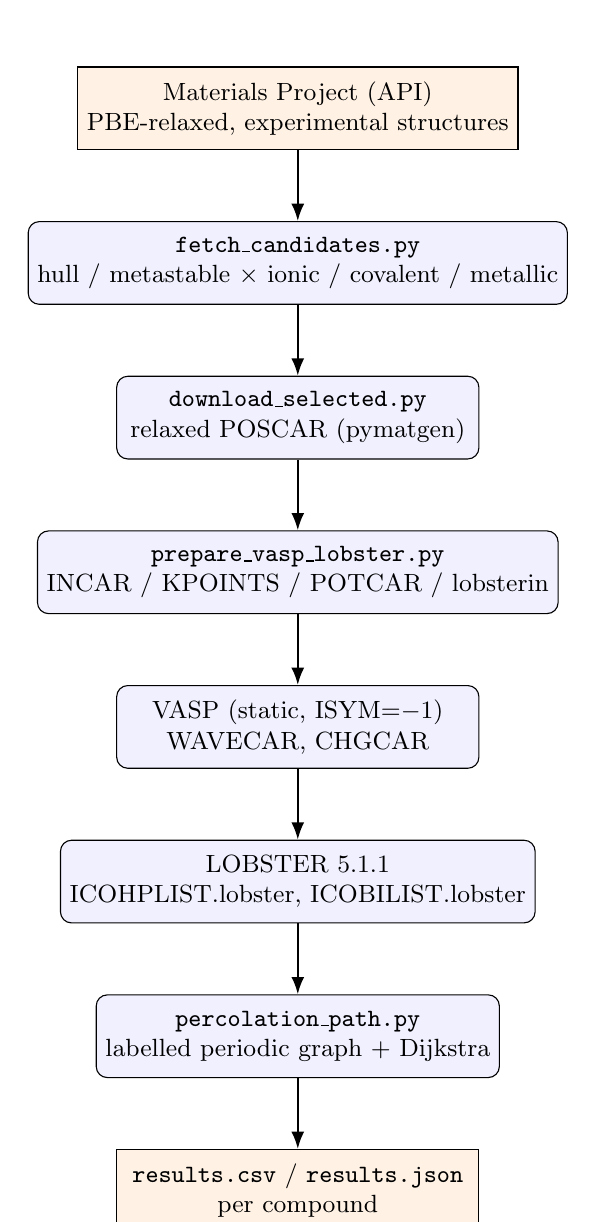
\begin{tikzpicture}[
  node distance=0.9cm and 1.6cm,
  box/.style={draw, rounded corners, minimum width=4.6cm, minimum height=1.05cm,
              align=center, fill=blue!6, font=\small},
  io/.style={draw, minimum width=4.6cm, minimum height=1.05cm, align=center,
             fill=orange!10, font=\small},
  arr/.style={-{Latex[length=2.2mm]}, thick}
]
\node[io]  (mp)     {Materials Project (API) \\ PBE-relaxed, experimental structures};
\node[box, below=of mp] (fetch)   {\texttt{fetch\_candidates.py} \\ hull / metastable $\times$ ionic / covalent / metallic};
\node[box, below=of fetch] (dl)     {\texttt{download\_selected.py} \\ relaxed POSCAR (pymatgen)};
\node[box, below=of dl] (prep)   {\texttt{prepare\_vasp\_lobster.py} \\ INCAR / KPOINTS / POTCAR / lobsterin};
\node[box, below=of prep] (vasp)   {VASP (static, ISYM=$-1$) \\ WAVECAR, CHGCAR};
\node[box, below=of vasp] (lob)    {LOBSTER 5.1.1 \\ ICOHPLIST.lobster, ICOBILIST.lobster};
\node[box, below=of lob] (perc)   {\texttt{percolation\_path.py} \\ labelled periodic graph + Dijkstra};
\node[io, below=of perc] (out)    {\texttt{results.csv} / \texttt{results.json} \\ per compound};

\draw[arr] (mp) -- (fetch);
\draw[arr] (fetch) -- (dl);
\draw[arr] (dl) -- (prep);
\draw[arr] (prep) -- (vasp);
\draw[arr] (vasp) -- (lob);
\draw[arr] (lob) -- (perc);
\draw[arr] (perc) -- (out);
\end{tikzpicture}
\end{center}

\section{Environment and Installation}

\subsection{Compute Machine}

The \textbf{Yargla} cluster (IC2MP, Université de Poitiers,
\texttt{yargla.chimie.univ-poitiers.fr}), SLURM scheduler, \texttt{defq}
partition.

\subsection{Software}

\begin{itemize}
  \item \textbf{VASP} 6.5.0 (module \texttt{vasp/6.5.0}), recommended
    PAW--PBE potentials per element.
  \item \textbf{LOBSTER} 5.1.1 (module \texttt{lobster/5.1.1}) --- the most
    recent version available on the cluster.
  \item \textbf{Python} 3.11, dedicated virtual environment
    \texttt{/home/gilles/viability/.venv}:
    \texttt{pymatgen} (structure analysis, LOBSTER parsing),
    \texttt{lobsterpy} (LOBSTER utilities),
    \texttt{mp-api} (Materials Project queries).
\end{itemize}

\subsection{Installation (Summary)}

\begin{lstlisting}
module load intel
module load impi/2021.13
module load vasp/6.5.0
module load lobster/5.1.1

python3.11 -m venv .venv
source .venv/bin/activate
pip install pymatgen lobsterpy mp-api
\end{lstlisting}

Each VASP+LOBSTER run is submitted through a SLURM script
(\texttt{submit.sh}, 1 node, 16 tasks, 24h max walltime), which chains
\texttt{vasp\_std} followed by \texttt{lobster-5.1.1} in the same working
directory.

\section{Dataset}

Six experimental (ICSD-referenced) compounds, PBE-relaxed by Materials
Project, $\leq 20$ atoms/cell, split into 2 families $\times$ 3 bonding
types:

\begin{center}
\begin{tabular}{@{}lllr@{}}
\toprule
Family & Bonding type & Compound (mp-id) & $E_\text{hull}$ (eV/atom) \\
\midrule
on hull       & ionic      & NaCl (mp-22862)               & 0.0000 \\
on hull       & covalent   & Si (mp-149)                   & 0.0000 \\
on hull       & metallic   & AlNi, B2 (mp-1487)            & 0.0000 \\
metastable    & ionic      & LiBr (mp-23259)                & 0.0099 \\
metastable    & covalent   & C, rhombohedral graphite (mp-169) & 0.0008 \\
metastable    & metallic   & BeCu (mp-2323)                 & 0.0050 \\
\bottomrule
\end{tabular}
\end{center}

\section{Results}

\begin{center}
\small
\begin{tabular}{@{}lrrrr@{}}
\toprule
Compound & Percolation weight & Direction & $\text{ICOHP}_\text{min}$ & $\text{ICOHP}_\text{mean}$ \\
        & (eV) & & (eV) & (eV) \\
\midrule
NaCl (hull, ionic)          & 0.0307 & $a$ & $-0.595$  & $-0.089$ \\
Si (hull, covalent)         & 0.0032 & $c$ & $-4.552$  & $-0.291$ \\
AlNi (hull, metallic)       & 0.0042 & $a$ & $-1.992$  & $-0.322$ \\
LiBr (metastable, ionic)         & 0.0988 & $c$ & $-2.041$  & $-0.338$ \\
C rhomb. (metastable, covalent)  & 0.0003 & $c$ & $-11.737$ & $-0.286$ \\
BeCu (metastable, metallic)      & 0.0005 & $b$ & $-1.848$ & $-0.162$ \\
\bottomrule
\end{tabular}
\end{center}

\section{Discussion: The Descriptor Diverges Sharply from Classic Aggregates}

The most striking result is that, for all six compounds, the percolation
weight is \textbf{one to four orders of magnitude smaller} than the
minimum ICOHP (strongest bond) and even than the mean ICOHP. This is
exactly the intended behavior: the percolation descriptor does not measure
the strength of the strongest bond, but the resistance of the
\emph{weakest} path that actually crosses the crystal --- and that path
does not necessarily use the strongest bonds available.

\textbf{Physical explanation for NaCl (representative case).} The
strongest Na--Cl bond ($-0.595$~eV) connects the two atoms \emph{within
the same primitive cell} (translation vector $(0,0,0)$): in the primitive
rhombohedral cell provided by Materials Project for this rock-salt-type
structure, this bond therefore crosses \emph{no} cell boundary and cannot
by itself contribute to a non-contractible cycle. The cheapest
non-contractible path instead uses second-coordination-shell Na--Na or
Cl--Cl interactions ($d \approx 3.95$~\AA, $|\text{ICOHP}| \approx
0.031$~eV), markedly weaker but which do actually cross a cell boundary
along the considered direction.

\textbf{Methodological implication.} This behavior is correct in the
strict sense of the requested topological definition (minimum-weight
non-contractible cycle over the \emph{primitive} lattice vectors), but it
means that the reported $a/b/c$ directions correspond to the primitive
cell vectors as supplied on input --- which, for high-symmetry structures
(rock-salt, zinc-blende, etc.), do not coincide with the conventional
crystallographic directions ($[100]$, $[010]$, $[001]$ cubic) one
intuitively pictures. For a reading directly comparable to conventional
axes, a natural extension would be to reconventionalize the cell (via
\texttt{pymatgen.symmetry.analyzer.SpacegroupAnalyzer.
get\_conventional\_standard\_structure}) before building the graph, or to
evaluate the minimum weight over a richer set of target vectors (simple
combinations of $a,b,c$); this was not done in this first pass but is
flagged here as a natural improvement.

This divergence nonetheless confirms the project's premise: the
percolation descriptor carries information \emph{qualitatively different}
from classic ICOHP aggregates, and is not redundant with them.

\section{Conclusion and Outlook}

The complete pipeline --- Materials Project query, LOBSTER-compatible
VASP calculation, and topologically exact percolation analysis without a
supercell --- was run end-to-end on six real compounds (3 on-hull, 3
experimental metastable), covering the three major bonding types (ionic,
covalent, metallic). The results confirm that the percolation descriptor
captures information distinct from the usual ICOHP/ICOBI aggregates.

Directions for future work: (i) cell reconventionalization before graph
construction, to align reported directions with the usual crystallographic
axes; (ii) extending the test set to several dozen compounds for a
statistical analysis; (iii) a sensitivity study with respect to the
upstream ICOHP/ICOBI cutoff radius.

\vspace{1cm}
\noindent\textit{Source code:} \url{https://github.com/John-Akapulco/viability}

\end{document}
